% =====================================================================
% main.tex - self-contained Overleaf-ready harness for methodology.tex
%
% Upload these four files to a single Overleaf project (flat structure):
%   main.tex                    <-- this file; set as "Main document"
%   methodology.tex
%   methodology_preamble.tex
%   references.bib
%
% Then build with pdfLaTeX.  Overleaf will run latex/bibtex/latex/latex
% automatically when you compile.
% =====================================================================

\documentclass[11pt]{article}

% ---------------------------------------------------------------------
% Page geometry (replace with your venue's class file when ready)
% ---------------------------------------------------------------------
\usepackage[margin=1in]{geometry}

% Scalable fonts must be loaded BEFORE microtype, otherwise pdfTeX
% throws "auto expansion is only possible with scalable" and aborts.
\usepackage[T1]{fontenc}
\usepackage{lmodern}
\usepackage{microtype}

% ---------------------------------------------------------------------
% Pull in everything methodology.tex requires
% ---------------------------------------------------------------------
% =====================================================================
% Preamble additions required to compile methodology.tex
% Drop these \usepackage{} lines into the main paper preamble (alongside
% whatever the venue template already loads).  None of these clash with
% standard NeurIPS / ICML / ACL / ICLR / arXiv class files.
% =====================================================================

% --- math ---
\usepackage{amsmath,amssymb,amsfonts}
\usepackage{amsthm}
\newtheorem{remark}{Remark}        % \begin{remark}[Optional title] ... \end{remark}
\newtheorem{proposition}{Proposition}
\newtheorem{definition}{Definition}

% --- citations ---
% natbib gives you \citep{} and \citet{} which the section uses.
% If your venue template already loads natbib (most ML/NLP templates do),
% delete this line; the \citep{} / \citet{} calls will work unchanged.
\usepackage[authoryear,round]{natbib}

% --- algorithm / pseudocode ---
\usepackage{algorithm}
\usepackage{algpseudocode}
% (algpseudocode replaces the older algorithmic package and supports
%  \Statex, \Comment, \Require, \Ensure used in Algorithm 1.)

% --- tables ---
\usepackage{booktabs}     % \toprule / \midrule / \bottomrule

% --- figures (TikZ + libraries the architecture diagram uses) ---
\usepackage{tikz}
\usetikzlibrary{
  positioning,
  shapes.geometric,        % diamond gate
  arrows.meta,             % stealth arrowheads
  calc,                    % $(node)+(...)$ coordinate arithmetic
  fit,                     % optional grouping boxes
  backgrounds              % optional layered backgrounds
}

% --- code-style fonts (\texttt is sufficient; nothing extra needed) ---

% --- optional: tighter equation spacing if your template is loose ---
% \setlength{\abovedisplayskip}{4pt plus 1pt minus 1pt}
% \setlength{\belowdisplayskip}{4pt plus 1pt minus 1pt}

% =====================================================================
% Notes on cross-references the section assumes you have defined
% somewhere in the paper:
%
%   \label{sec:intro}        in Section 1 (Introduction)
%   \label{sec:experiments}  in Section 4 (Experiments)
%
% The methodology file itself defines every other label it references.
% =====================================================================


% ---------------------------------------------------------------------
% Hyperlinks (load LAST in the preamble - this is a hard rule for natbib)
% ---------------------------------------------------------------------
\usepackage[hidelinks]{hyperref}

% =====================================================================
\begin{document}
% =====================================================================

\title{Compiled Reward Systems for Open-Ended Reinforcement Learning}
\author{Anonymous}
\date{}
\maketitle

% ---------------------------------------------------------------------
% Section 1 - Introduction (placeholder so \ref{sec:intro} resolves)
% ---------------------------------------------------------------------
\section{Introduction}
\label{sec:intro}

\textit{Placeholder.}  Replace this section with the introduction draft.
The methodology in Section~\ref{sec:methodology} references this
section's \texttt{sec:intro} label, so the label must exist.

% ---------------------------------------------------------------------
% Section 2 - Related Work (optional; safe to delete)
% ---------------------------------------------------------------------
\section{Related Work}
\label{sec:related}

\textit{Placeholder.}

% ---------------------------------------------------------------------
% Section 3 - Methodology (this is the actual section file)
% ---------------------------------------------------------------------
% =====================================================================
% Section 3 - Methodology  (descriptive, pipeline-detailed; under 4 pages)
% Method tone; two-phase framing (compile-time / inference-time).
% =====================================================================

\section{Methodology}
\label{sec:methodology}

\subsection{Problem setup}
\label{sec:problem-setup}

Let $x \in \mathcal{X}$ denote a prompt and $y \in \mathcal{Y}$ a candidate
response in a domain where no executable verifier exists for the full
task.  Compositional Rubric Refinement (CRR) defines a \emph{compiled
reward}
%
\begin{equation}
\label{eq:compiled-reward}
r(x, y) \;=\; \Phi\!\Big(
  S_{\mathcal{G}}(x, y),\;
  \{V_k(x, y)\}_{k\in\mathcal{V}(x)},\;
  \mathcal{H}(x, y)
\Big),
\end{equation}
%
where $S_{\mathcal{G}}$ is a learned rubric score on a rubric set
$\mathcal{G}$, $\{V_k\}_{k\in\mathcal{V}(x)}$ is a task-family-routed
collection of deterministic and independent verification signals,
$\mathcal{H}$ is a vector of hard-gate predicates, and $\Phi$ is a
deterministic composition map (\S\ref{sec:phi}).  For pairwise
evaluation we instantiate Eq.~\eqref{eq:compiled-reward} on $(y_A, y_B)$
to produce a verdict $V \in \{A{\succ}B,B{\succ}A,A{=}B\}$; for direct
supervision each rollout is scored independently with the same
machinery.  Each criterion
$g_k\!:\!\mathcal{X}{\times}\mathcal{Y}{\to}\{0,1\}$ carries a
non-negative weight $w_k$, a severity tier
$\tau_k \in \{\textsc{cat},\textsc{ess},\textsc{imp},\textsc{opt}\}$, a
verdict in
$\{\textsc{met},\textsc{unmet},\textsc{n/a},\textsc{cannot\_assess}\}$,
and one or more evidence anchors.  In the standard rubric-as-reward
formulation \citep{gunjal2025rar}, $\Phi$ collapses to a normalized
weighted sum $\sum_k w_k g_k$ with $\mathcal{V}(x){=}\emptyset$ and
$\mathcal{H}{\equiv}0$.

\subsection{Architecture overview}
\label{sec:architecture}

CRR is organized as three composed layers (Fig.~\ref{fig:architecture}).
The \textbf{rubric layer} (\S\ref{sec:rubric-layer}) induces
broad-coverage, instance-specific evaluation criteria, scores them,
and emits a pair-level discriminator verdict.  The \textbf{verification
layer} (\S\ref{sec:verifiers}) runs task-family-routed deterministic
and independent procedures that emit sparse, high-precision signals.
The \textbf{composition map} $\Phi$ (\S\ref{sec:phi}) deterministically
combines them via the procedure of Algorithm~\ref{alg:override} and
emits a final verdict together with an audit-trail
\texttt{decision\_source}.  The three-layer division reflects the
structure of evidence in non-verifiable evaluation: the rubric layer
provides broad but noisy coverage of quality dimensions, the
verification layer provides sparse but high-precision signal where
structure permits, and the composition map combines them under
principled disagreement-resolution; no single layer is sufficient.
CRR's central methodological claim is that compiling rubric-induction
artifacts offline and combining them with family-routed independent
verification through a deterministic composition map produces a
reward signal whose accuracy in pairwise evaluation improves over
any single-source rubric reward, while preserving the simpler
rubric-only score as a fallback for direct supervision.

\paragraph{Two phases.}
The framework operates in two phases sharing the same rubric-induction
machinery.  At \textbf{compile time}, CRR runs the induction machinery
(\S\ref{sec:rubric-layer}) over a compilation corpus to distill a
task-family-keyed rubric library, calibrates per-verifier confidence
thresholds and HP-set membership, and binds the resulting artifacts
into a \emph{frozen policy hash}.  At \textbf{inference time}, on each
new prompt, CRR runs the same induction machinery to discover
prompt-local criteria, retrieves complementary criteria from the
frozen library, and routes the discriminator verdict through the
verification layer and composition map.  Persisting the inductive
artifacts at compile time keeps the inference pass cheap and
reproducible; no hyperparameter is selected on a held-out split, and
no per-pair tuning is permitted at inference.

% --------------------------------------------------------------------
% Figure 1 - System architecture (TikZ)
% --------------------------------------------------------------------
\begin{figure}[!t]
\centering
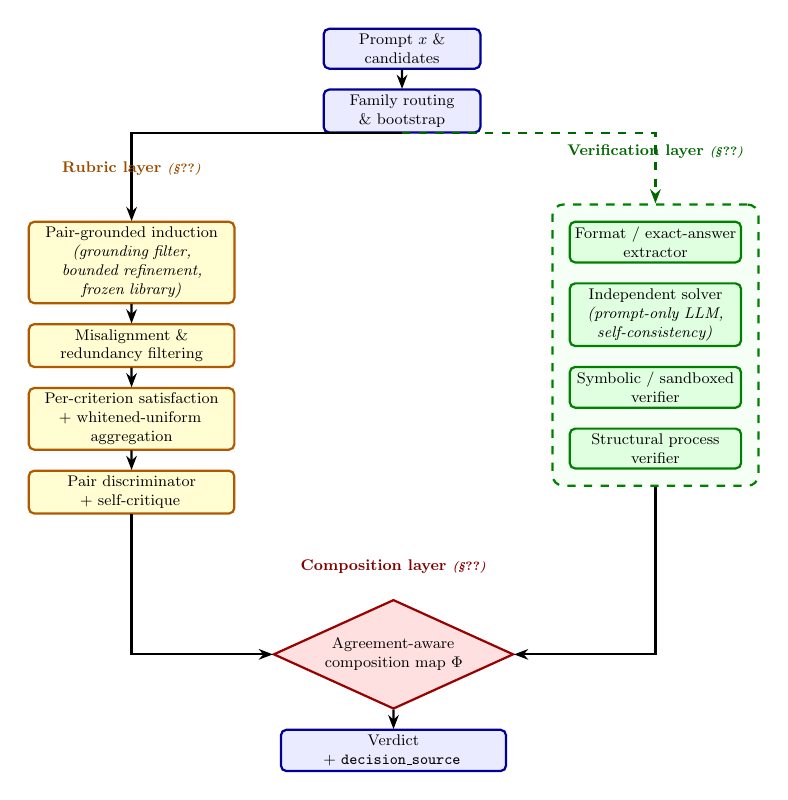
\begin{tikzpicture}[
    scale=0.62, transform shape,
    font=\small,
    >={Stealth[length=1.8mm]},
    node distance=4mm and 6mm,
    every node/.style={align=center},
    box/.style={rectangle, rounded corners=2pt, draw, thick,
                inner sep=3pt, minimum height=7mm, text width=30mm},
    inputbox/.style={box, fill=blue!8,    draw=blue!60!black},
    rubricbox/.style={box, fill=yellow!18, draw=orange!70!black, text width=40mm},
    verifybox/.style={box, fill=green!12,  draw=green!50!black, text width=33mm},
    gatebox/.style={diamond, draw, thick, fill=red!12, draw=red!60!black,
                    aspect=2.2, inner sep=2pt, text width=30mm},
    grouptitle/.style={font=\small\bfseries, anchor=south}
]
  \node[inputbox]                 (input)  {Prompt $x$ \& candidates};
  \node[inputbox, below=of input] (route)  {Family routing\\\& bootstrap};

  \node[rubricbox, below left=18mm and 18mm of route] (disc)
        {Pair-grounded induction\\\textit{(grounding filter,\\bounded refinement,\\frozen library)}};
  \node[rubricbox, below=of disc] (filt)
        {Misalignment \&\\redundancy filtering};
  \node[rubricbox, below=of filt] (agg)
        {Per-criterion satisfaction\\$+$ whitened-uniform aggregation};
  \node[rubricbox, below=of agg]  (disc2)
        {Pair discriminator\\$+$ self-critique};

  \node[verifybox, below right=18mm and 18mm of route] (vexact)
        {Format / exact-answer\\extractor};
  \node[verifybox, below=of vexact] (vsolver)
        {Independent solver\\\textit{(prompt-only LLM,}\\\textit{self-consistency)}};
  \node[verifybox, below=of vsolver] (vsymbolic)
        {Symbolic / sandboxed\\verifier};
  \node[verifybox, below=of vsymbolic] (vstruct)
        {Structural process\\verifier};

  \begin{scope}[on background layer]
    \node[draw=green!50!black, dashed, rounded corners=4pt,
          fit=(vexact)(vstruct), inner sep=6pt, thick,
          fill=green!4] (vgroup) {};
  \end{scope}

  \node[gatebox, below=22mm of $(disc2.south)!0.5!(vstruct.south)$] (gate)
        {Agreement-aware\\composition map $\Phi$};
  \node[inputbox, below=of gate, text width=44mm] (out)
        {Verdict\\$+$ \texttt{decision\_source}};

  \draw[->, thick] (input) -- (route);
  \draw[->, thick] (route.south) -| (disc.north);
  \draw[->, thick] (disc)  -- (filt);
  \draw[->, thick] (filt)  -- (agg);
  \draw[->, thick] (agg)   -- (disc2);

  \draw[->, thick, dashed, draw=green!40!black]
       (route.south) -| (vgroup.north);

  \draw[->, thick] (disc2.south)  |- (gate.west);
  \draw[->, thick] (vgroup.south) |- (gate.east);

  \draw[->, thick] (gate.south) -- (out.north);

  \node[grouptitle, text=orange!60!black]
        at ($(disc.north)+(0,8mm)$)
        {\textsc{Rubric layer} \scriptsize\textit{(\S\ref{sec:rubric-layer})}};
  \node[grouptitle, text=green!40!black]
        at ($(vgroup.north)+(0,8mm)$)
        {\textsc{Verification layer} \scriptsize\textit{(\S\ref{sec:verifiers})}};
  \node[grouptitle, text=red!50!black]
        at ($(gate.north)+(0,4mm)$)
        {\textsc{Composition layer} \scriptsize\textit{(\S\ref{sec:phi})}};
\end{tikzpicture}

\caption{\emph{CRR architecture.}  The rubric layer (yellow) produces
a discriminator verdict; the verification layer (green) runs
task-family-routed verifiers that observe the prompt only, never both
candidates (dashed arrow); the composition map $\Phi$ (red) combines
the two via Algorithm~\ref{alg:override}.}
\label{fig:architecture}
\end{figure}

\subsection{Rubric layer}
\label{sec:rubric-layer}

The rubric layer maps a prompt $x$ and candidate set
$\{y_1, \ldots, y_n\}$ to a per-criterion satisfaction matrix
$M \in \{0,1\}^{n \times m}$, weights $w \in \mathbb{R}^m_+$, and a
pair-level discriminator verdict $D_{\text{rub}}$.  Stages~1--6 below
constitute the induction machinery shared by both phases; stages~7--8
are inference-time scoring.

\paragraph{Task-family routing.}
Each prompt is routed to a task profile drawn from a finite registry
of profiles indexed by task family.  Unfamiliar prompts trigger an
automatic bootstrap that synthesizes a temporary profile rather than
forcing a poor static fit.  Each profile carries a discovery-dimension
list, a contrast-strategy preference, and a source-priority ordering
for selecting the strong anchor; this ensures that downstream stages
operate on inputs adapted to the family's quality conventions rather
than on a generic template.

\paragraph{Contrast pair construction.}
For each example we form one or more strong/weak pairs $(y_s, y_w)$.
The strong anchor $y_s$ is selected by source priority -- typically a
reference completion or, when unavailable, the strongest
writer-generated candidate -- and the weak side $y_w$ is either an
alternative completion or a profile-specific structured mutation
targeting one dominant failure mode (omission, hallucination,
certainty inflation, structure drop, plan drop).  Polarity is
required: without an explicit strong/weak designation, the proposer
has no signal for what \emph{distinguishes} good from bad in the
instance, and the grounding test of the next stage is not defined.

\paragraph{Initial proposal.}
A single LLM call per pair emits a small set of atomic criteria
following the desiderata of \citet{gunjal2025rar}: each criterion
must be expert-grounded, comprehensive, importance-weighted, and
self-contained, and must carry a dimension label, a severity tier
$\tau_k$, and a binary-leaning one-sentence requirement.  Proposers
are alternated across pairs to diversify the rubric set and reduce
proposer-style bias in the resulting bank.

\paragraph{Pair-grounding test and bounded decomposition.}
Each proposed criterion passes a deterministic check that its
requirement text lexically aligns with the strong-vs-weak delta and,
when the weak side is synthetic, with the active mutation profile;
failed proposals are preserved in a per-pair audit log so the
rejection ratio is inspectable.  Surviving criteria with overly broad
coverage are then submitted for one round of narrower-child
decomposition under a bounded budget
$(\texttt{depth},\,\texttt{parents/pair},\,\texttt{children/parent},\,\texttt{calls/pair}) = (1, 2, 3, 2)$,
with the parent retained whenever no child survives.  Bounding the
recursion at depth one is deliberate: deeper decomposition compounds
proposer noise faster than it improves granularity.

\paragraph{Frozen library retrieval (compile-time artifact).}
At compile time the induction outputs are aggregated by task family
into a frozen rubric library that ships with the locked policy.  At
inference time the library is consulted by TF-IDF retrieval over the
prompt with top-$k{=}6$ in family-strict mode.  This compile-once,
retrieve-many design decouples coverage from per-prompt induction
cost: prompt-local discovery is sample-efficient but coverage-limited
on individual prompts, while the precompiled library injects criteria
the proposer would not have produced for this specific pair.

\paragraph{Misalignment and redundancy filtering.}
The merged proposal pool -- prompt-local plus retrieved -- is filtered
at aggregation time rather than at criterion-deletion time.  A
\emph{misalignment filter} discards any criterion whose requirement
text would, read literally, favor the weaker side of an originating
pair; a \emph{redundancy filter} greedily Jaccard-clusters criteria on
requirement+label+dimension tokens with threshold $0.9$ and retains
the highest-severity representative per cluster.  Both filters are
deterministic and audit-trailed.

\paragraph{Per-criterion satisfaction.}
Surviving criteria are evaluated by a single LLM call per
$(g_k, y_i)$ pair using GPT-4o, sampled at $N{=}1$, $T{=}0$.  The
judge emits a verdict in the four-class vocabulary of
\S\ref{sec:problem-setup}; malformed outputs are mapped to
\textsc{cannot\_assess} \citep{rao2026autorubric} and score as $0$ to
prevent unparseable verdicts from inflating soft scores.  In our
setting, $N{=}1$ at $T{=}0$ outperforms multi-sample self-consistency
at the per-criterion level -- in contrast to the discriminator and
solver layers, where multi-sampling is positive (\S\ref{sec:verifiers},
\S\ref{sec:rubric-layer}); we report this ablation in
\S\ref{sec:experiments}.

\paragraph{Whitened-uniform aggregation and discriminator.}
With satisfaction matrix $M$, weights are assigned by whitened-uniform
aggregation: $\Sigma = \mathrm{Cov}(M) + \lambda I$ with
$\lambda{=}10^{-3}$, and $w = \Sigma^{-1/2}\mathbf{1}$, clipped
non-negative and renormalized.  This adopts the correlation-aware
aggregation of \citet{shen2026rrd}, which minimizes the
misclassification upper bound
%
\begin{equation}
\label{eq:wu-bound}
\Pr(\hat{Y}\neq Y) \;\leq\;
\exp\!\left(-\tfrac{1}{2}\,\frac{(w^{\!\top}\!\mu)^{2}}{w^{\!\top}\Sigma\,w}\right),
\end{equation}
%
where $\mu$ is the per-criterion edge over chance.  Per-candidate
scores $S_{\mathcal{G}}(x, y_i) = \sum_k w_k\, M_{ik}$ are then
consumed by a pair discriminator: a single GPT-4o call observes both
candidates and the WU scores and emits $A{\succ}B$, $B{\succ}A$, or
$A{=}B$ under self-consistency $(N, T){=}(5, 0.7)$ with majority
voting.  A second pass critiques the first verdict and may reverse
it; the critique addresses the regime in which discriminator errors
cluster -- low-margin pairs where the first call's quick judgement is
most unreliable.

\subsection{Verification layer}
\label{sec:verifiers}

The verification layer routes a prompt of family $\mathrm{fam}(x)$ to
a family-specific subset $\mathcal{V}(x) \subseteq \mathcal{V}$
spanning four classes.  \textbf{Format / exact-answer extractors}
parse the candidate's final-answer region and compare against a
parseable target.  \textbf{Independent solvers} are separate strong
LLMs, distinct from the discriminator, that observe the prompt only
and emit an answer whose canonicalized form is compared against each
candidate.  \textbf{Symbolic and sandboxed verifiers} include
computer-algebra checks, subprocess Python execution against test
harnesses, and class-method test runners.  \textbf{Structural process
verifiers} are hand-crafted checks for task-completeness or internal
consistency that are too brittle for LLMs but cheap and reliable on a
fixed family.

Each verifier emits a uniform outcome -- a triggered flag, a
recommended decision, a confidence in
$\{\textsc{low},\textsc{med},\textsc{high}\}$, and a margin -- with
confidence calibrated on the compilation corpus.  Free-form solvers
run with self-consistency $N{=}3$ at $T{=}0.5$ (higher than the
per-criterion satisfaction layer because free-form generation has
higher token-level variance and benefits from majority-vote
canonicalization of its emitted answer); deterministic verifiers run
at $N{=}1$.  The prompt-only access discipline is essential: a
verifier that observed both candidates would re-introduce the
discriminator's bias rather than inject orthogonal evidence, the
same discipline used by \citet{shen2026rrd} for sample-response
generators.  A verifier is admitted to the \emph{high-precision}
(HP) set $\mathcal{V}_{\text{HP}}$ only if its measured precision on
the compilation corpus exceeds an admission threshold (we use
$0.80$, the value above which an override is expected to be
net-positive against the rubric layer's baseline accuracy on the
compilation corpus); verifiers below the bar remain in $\mathcal{V}$
but are gated behind a margin rule and never trigger overrides.

\subsection{The composition map $\Phi$}
\label{sec:phi}

The composition map $\Phi$ in Eq.~\eqref{eq:compiled-reward} is the
deterministic procedure of Algorithm~\ref{alg:override}, taking the
rubric-layer verdict $D_{\text{rub}}$, the exact-answer extractor
verdict $D_{\text{exact}}$ (or $\bot$ when no extractor applies), and
the HP-verifier outcomes $\{V_k\}$ as input, and returning a verdict
together with a single decision source $s$.

\begin{algorithm}[t]
\caption{Agreement-aware composition map $\Phi$}
\label{alg:override}
\begin{algorithmic}[1]
\Require $D_{\text{rub}}$;\, $D_{\text{exact}} \in \{A{\succ}B,B{\succ}A,A{=}B,\bot\}$;\,
         $\{V_k\}_{k\in\mathcal{V}_{\text{HP}}}$.
\Ensure  Verdict $V^{\star}$, source $s$.
\For{$k \in \mathcal{V}_{\text{HP}}$}
  \If{$V_k.\textsc{trig}\,\wedge\, V_k.\textsc{conf}{=}\textsc{high}\,\wedge\,
       V_k.\textsc{rec}\!\neq\!D_{\text{rub}}$}
    \State \Return $(V_k.\textsc{rec},\, k)$ \Comment{R1: explicit override}
  \EndIf
\EndFor
\If{$D_{\text{exact}} \neq \bot$}
  \For{$k \in \mathcal{V}_{\text{HP}}$}
    \If{$V_k.\textsc{trig}\,\wedge\, V_k.\textsc{conf}{=}\textsc{high}\,\wedge\,
         V_k.\textsc{rec}\!=\!D_{\text{exact}}$}
      \State \Return $(D_{\text{exact}},\, \texttt{exact}{\oplus}k)$
                \Comment{R2: agreement-aware}
    \EndIf
  \EndFor
\EndIf
\State \Return $(D_{\text{rub}},\, \texttt{rubric})$ \Comment{R3: default}
\end{algorithmic}
\end{algorithm}

\noindent
The procedure characterizes three regimes for combining the rubric
layer with the verification layer.  \textbf{R1} is the explicit
override path: when an HP verifier disagrees with the rubric verdict
at \textsc{high} confidence, the verifier wins -- conservative by
design, since the rubric layer carries the broadest signal across the
candidate space and is the safest default whenever no high-precision
evidence is available.  \textbf{R2}, the agreement-aware path, fires
when the format-based exact-answer extractor and an HP verifier
independently arrive at the same recommendation; concurrence between
two procedures with orthogonal noise profiles is a high-precision
signal in its own right, since the joint event is rare under any
null hypothesis in which the procedures are independent.
\textbf{R3} is the safe default.  Hard-gate predicates $\mathcal{H}$
apply \emph{before} $\Phi$ as a deterministic eligibility filter:
catastrophic-tier criteria disqualify a candidate before it reaches
the composition map, preventing catastrophic failures from being
averaged away by soft criteria \citep{bai2022constitutional}.

\paragraph{Output semantics and downstream use.}
$\Phi$ returns a $(\text{verdict}, \text{decision\_source})$ pair.
The verdict is consumed directly when CRR is used as a pairwise
preference judge.  When CRR is used as a scalar reward signal -- for
example, in reinforcement fine-tuning over single-completion rollouts
-- the underlying signal is the WU-weighted score
$S_{\mathcal{G}}(x, y)$ for gate-passing candidates and a designated
penalty value otherwise; HP overrides apply only in the pairwise
case, where two candidates are available for $\Phi$ to discriminate.
The decision source field, recorded on every output, supports
per-component attribution analysis: it identifies which of R1, R2, or
R3 produced the verdict and, in the override cases, which verifier
$k$ supplied the override.  This decomposition is what makes the
composition layer auditable, and it is the basis on which we can
report (in \S\ref{sec:experiments}) that a non-trivial fraction of
correct verdicts are resolved by HP overrides rather than by the
rubric layer alone.

\paragraph{Determinism.}
$\Phi$ adds no LLM calls beyond those already required by the rubric
and verification layers; conditional on the layer outputs and the
frozen policy hash, the entire reward $r(x, y)$ is deterministic.



% ---------------------------------------------------------------------
% Section 4 - Experiments (placeholder so \ref{sec:experiments} resolves)
% ---------------------------------------------------------------------
\section{Experiments}
\label{sec:experiments}

\textit{Placeholder.}  Replace this section with the experiments draft.
The methodology references this section's \texttt{sec:experiments} label.

% ---------------------------------------------------------------------
% Bibliography
% ---------------------------------------------------------------------
\bibliographystyle{plainnat}
\bibliography{references}

% =====================================================================
\end{document}
% =====================================================================
